\documentclass{beamer}
\usetheme{ConnectivityLab}
\usepackage{times}
\usepackage{graphicx}
\usepackage{verbatim}
\usepackage{outlines}
\usepackage{fancyhdr}
\usepackage{subfigure}
\usepackage{cancel}
\usepackage{bibentry}
\usepackage{varwidth}
\usepackage{etoolbox}
\usepackage{epstopdf}
%%%%%%%%%%%%%%%%%%%%%%%%%%%%%%%%%%%%%%%%%%%%%%%%%%%%%%
%%%%%%%%%%%%%%%%%%%%%%%%%%%%%%%%%%%%%%%%%%%%%%%%%%%%%%

\title {
    Optimal Resource Dedication in Grouped Random Access for Massive Machine-Type Communications ~\cite{1707.09811}
}
\author {
    Yin-Hong Hsu
}
\date {
    08 24, 2017
}

%%%%%%%%%%%%%%%%%%%%%%%%%%%%%%%%%%%%%%%%%%%%%%%%%%%%%%
%%%%%%%%%%%%%%%%%%%%%%%%%%%%%%%%%%%%%%%%%%%%%%%%%%%%%%

\begin{document}
\begin{frame}
    \titlepage
\end{frame}

%%%%%%%%%%%%%%%%%%%%%%%%%%%%%%%%%%%%%%%%%%%%%%%%%%%%%%
%%%%%%%%%%%%%%%%%%%%%%%%%%%%%%%%%%%%%%%%%%%%%%%%%%%%%%

\begin{frame}{Outline}
    \tableofcontentsgather
    \tableofcontents
\end{frame}

%%%%%%%%%%%%%%%%%%%%%%%%%%%%%%%%%%%%%%%%%%%%%%%%%%%%%%
%%%%%%%%%%%%%%%%%%%%%%%%%%%%%%%%%%%%%%%%%%%%%%%%%%%%%%
\section{Introduction}
\begin{frame} {Background}
    \begin{itemize}
        \item {To Support massive Machine Type Communication (mMTC), Radio Access Network congestion is one of the most important issue.}
        \item {RAN congestions are caused by Random Access collisions}
    \end{itemize}
\end{frame}
\begin{frame} {Random Access Procedure}  
    \begin{figure}[t]
    \centering
    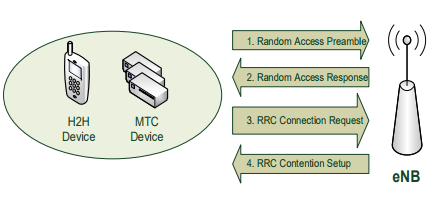
\includegraphics[width=0.8\textwidth]{figures/RAP.png}
    \setbeamerfont{caption}{size=\tiny}
    \end{figure}
\end{frame}
\begin{frame} {RA resource seperation}
    \begin{itemize}
        \item {The RA resource seperation scheme is different to ACB.}
        \item {It can decouple the collision rate problem between HTC and MTC.}
    \end{itemize}
\end{frame}
\begin{frame}   
    \begin{figure}[t]
    \centering
    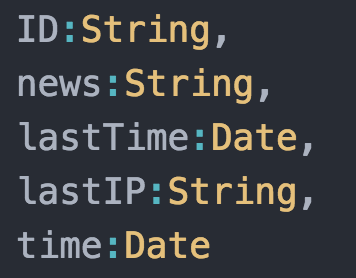
\includegraphics[width=1\textwidth]{figures/1.png}
    \setbeamerfont{caption}{size=\tiny}
    \end{figure}
\end{frame}
\begin{frame} {Grouped RA}
    \begin{itemize}
        \item {This study is based on D2D-based grouped RA}
        \item {Each group with a GC and several GM}
        \item {The group is clustered by device class (DC)}
    \end{itemize}
\end{frame}
\begin{frame} {Grouped RA}
    \begin{figure}[t]
    \centering
    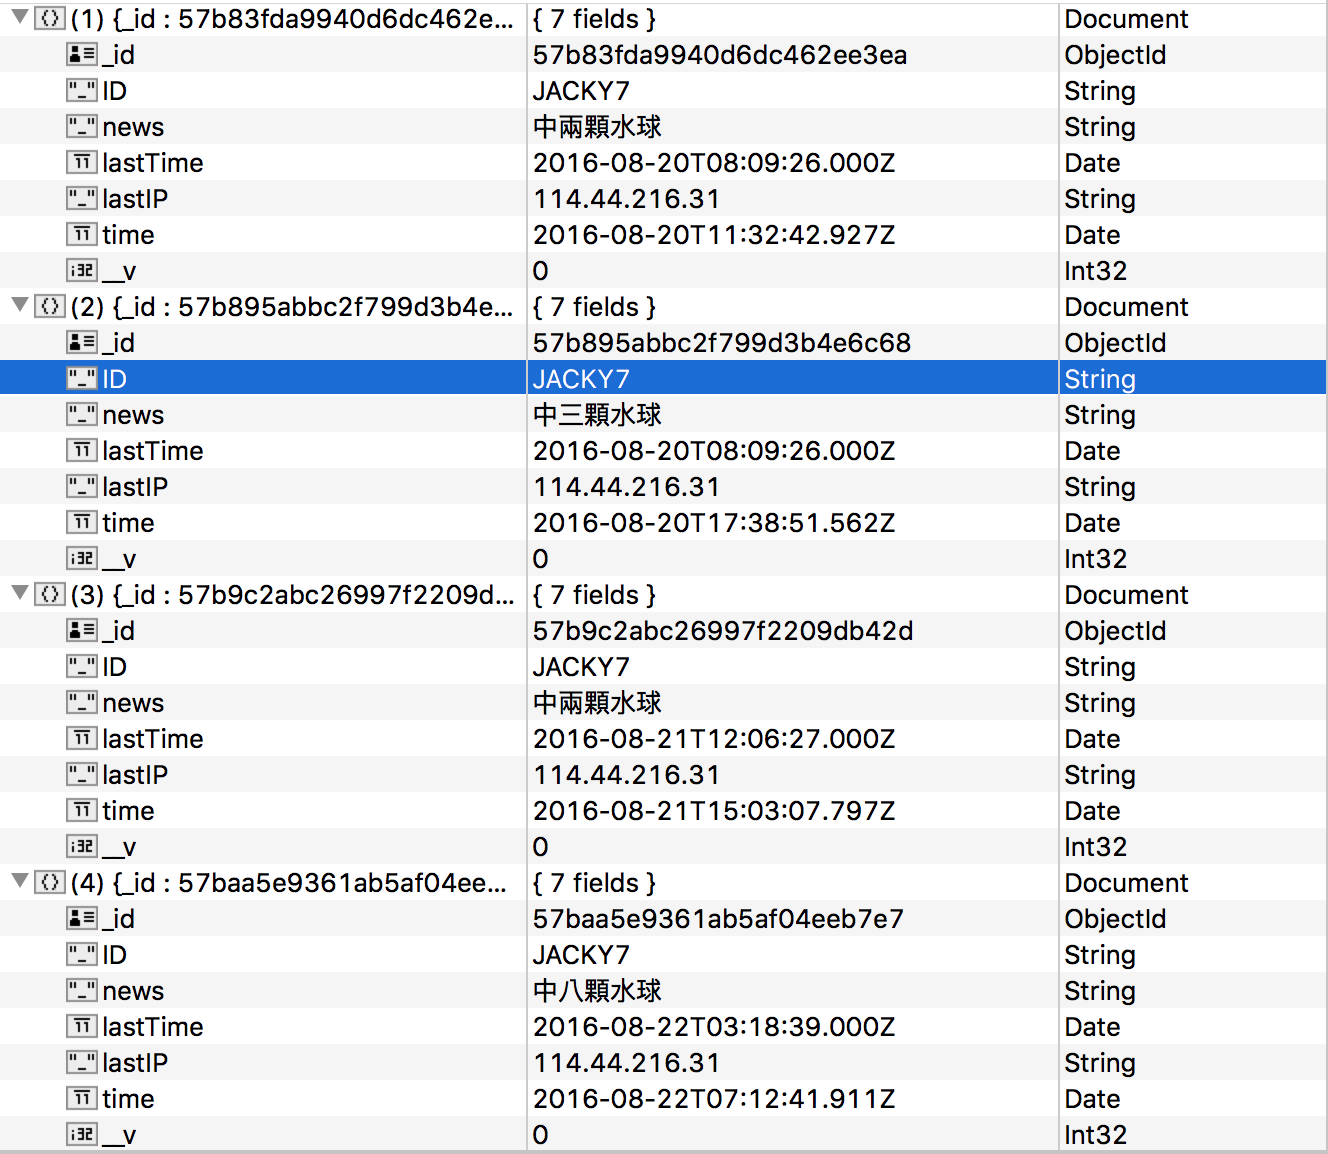
\includegraphics[width=0.8\textwidth]{figures/2.png}
    \setbeamerfont{caption}{size=\tiny}
    \end{figure}
\end{frame}
\section{Resource Allocation In Grouped Random Access}
\begin{frame} {Allocation strategy}
    \begin{itemize}
        \item {RACH resource can be flexibly allocate to different DC}
        \item {The allocation strategy can be concluded into three category}
        \begin{itemize}
            \item [-] {full sharing}
            \item [-] {full dedication}
            \item [-] {partial dedication}
        \end{itemize}
    \end{itemize}
\end{frame}
% \section{Collision Under Different Resource Allocation Strategies}
% \begin{frame}{}
% \end{frame}
\section{Optimized Random Access Channel Resource}
\begin{frame} {Allocation strategy}
    \begin{itemize}
        \item {Full sharing strategy is inflexible.}
        \item {This work is focus on full dedicate way.}
    \end{itemize}
\end{frame}
\begin{frame}{parameter in the algorithm}
    \begin{itemize}
        \item {L: number of RAOs}
        \item {N: number of classes}
        \item {$r_i$: average RA requests for each DC}
        \item {$\rho_i$: collision rate for each DC}
    \end{itemize}
\end{frame}
\begin{frame}
    \begin{figure}[t]
    \centering
    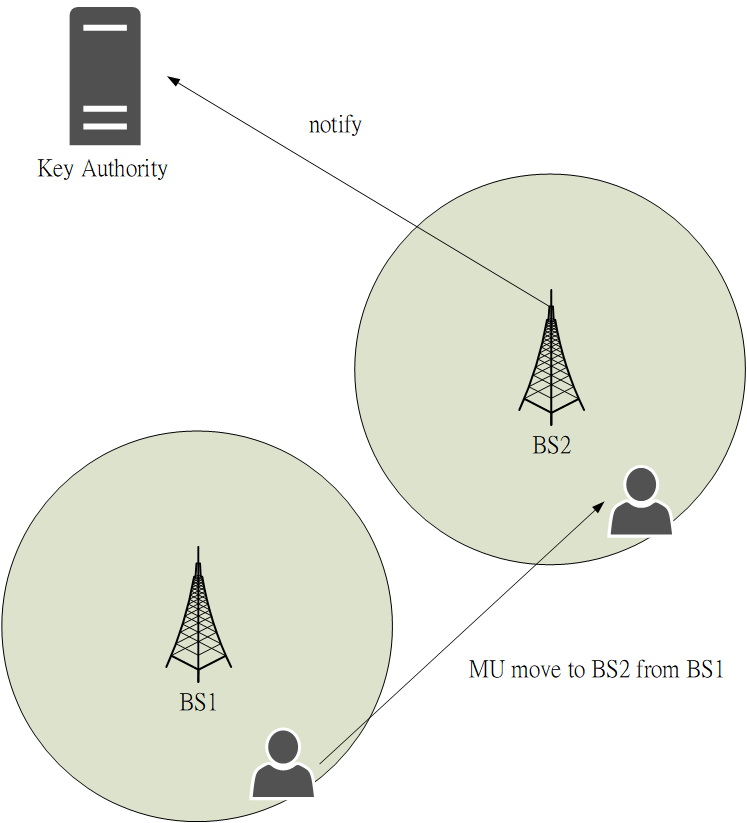
\includegraphics[width=1\textwidth]{figures/3.png}
    \setbeamerfont{caption}{size=\tiny}
    \end{figure}
\end{frame}
\section{Simulation}
\begin{frame}{}
    \begin{figure}[t]
    \centering
    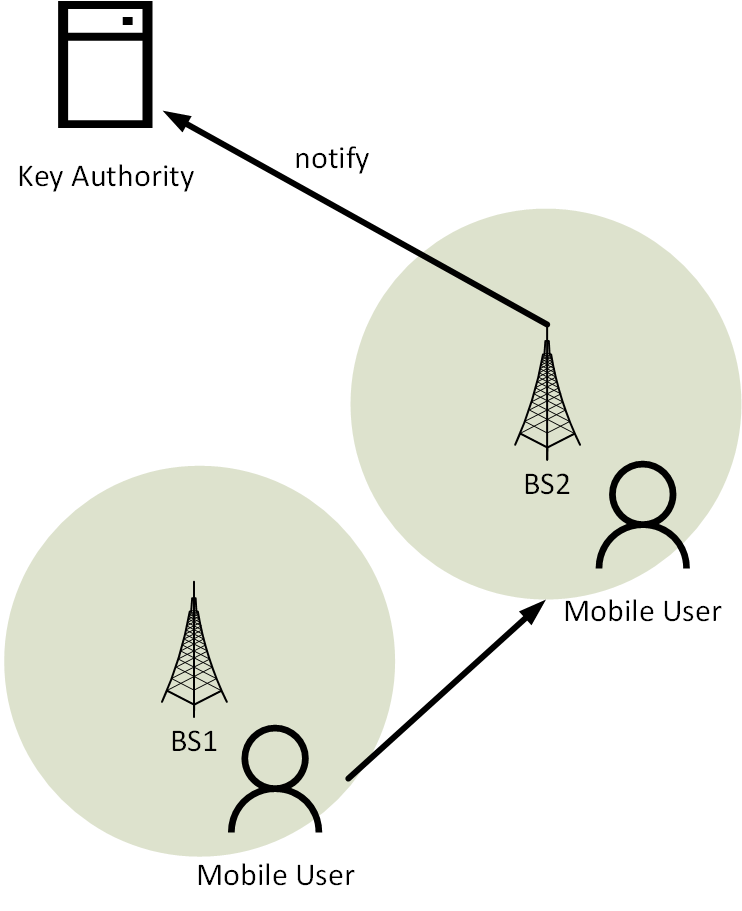
\includegraphics[width=1\textwidth]{figures/4.png}
    \setbeamerfont{caption}{size=\tiny}
    \end{figure}
\end{frame}
\begin{frame}{}
    \begin{figure}[t]
    \centering
    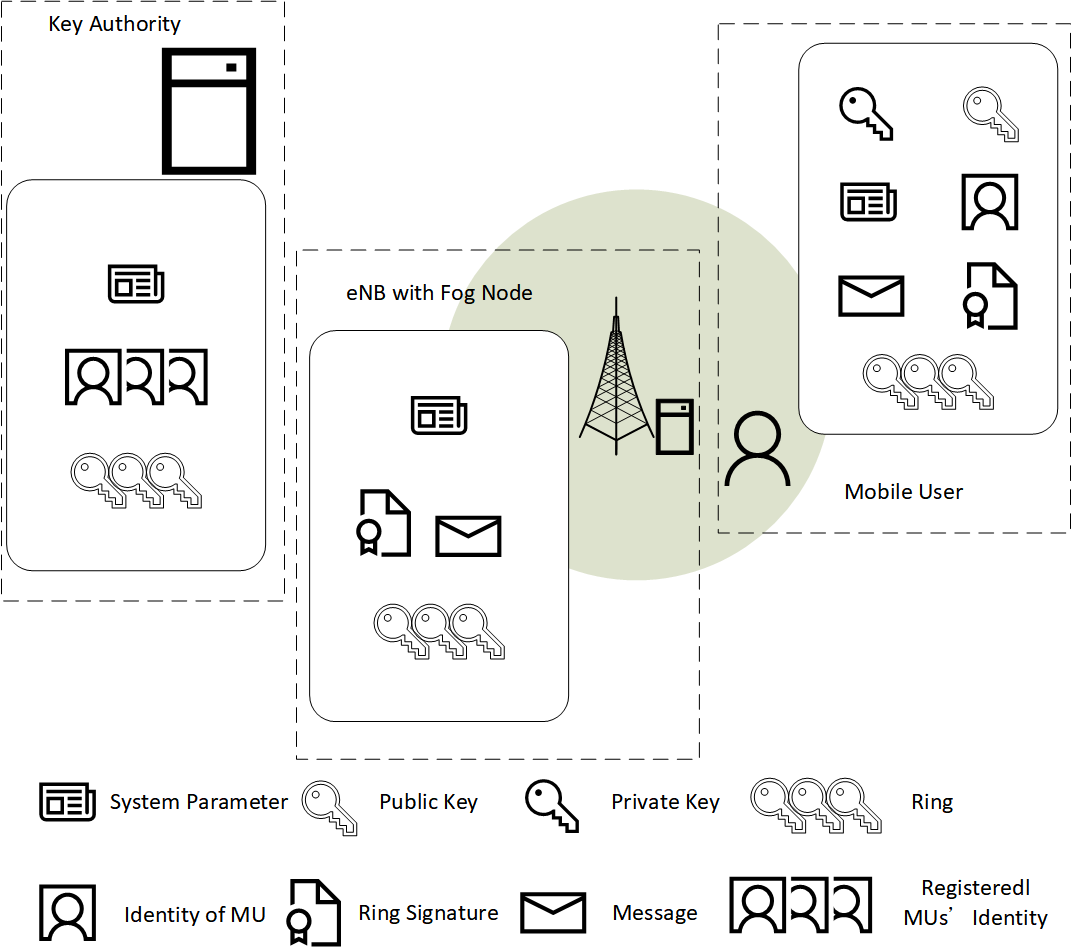
\includegraphics[width=1\textwidth]{figures/5.png}
    \setbeamerfont{caption}{size=\tiny}
    \end{figure}
\end{frame}
\begin{frame}{}
    \begin{figure}[t]
    \centering
    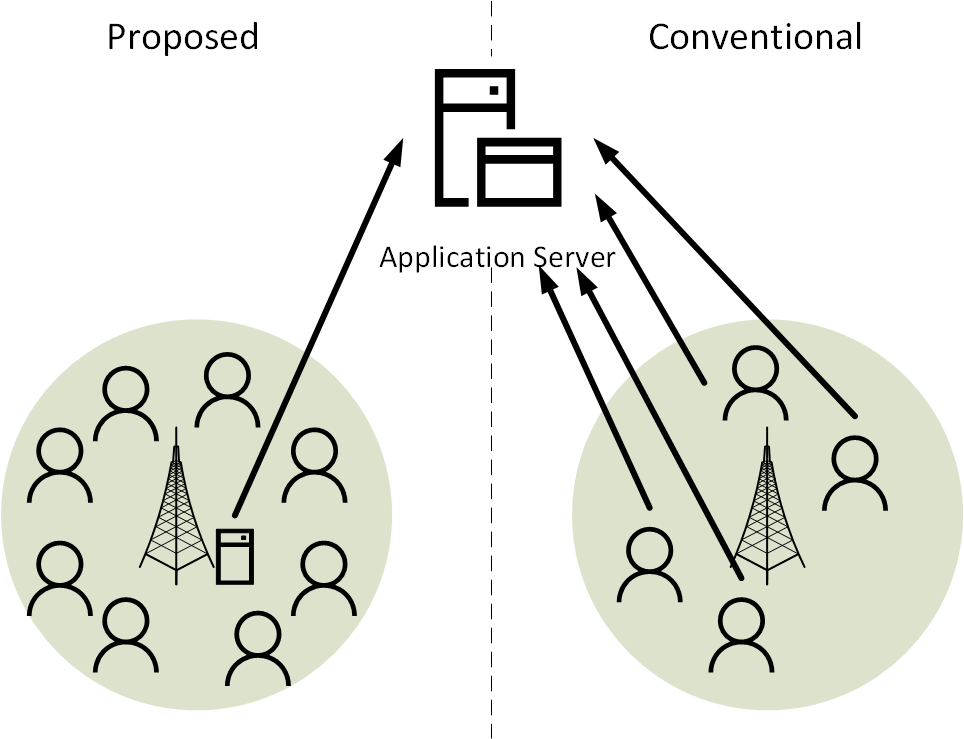
\includegraphics[width=1\textwidth]{figures/6.png}
    \setbeamerfont{caption}{size=\tiny}
    \end{figure}
\end{frame}
\begin{frame}{}
    \begin{figure}[t]
    \centering
    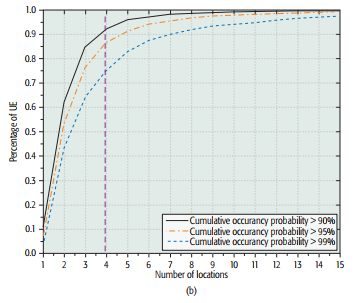
\includegraphics[width=1\textwidth]{figures/7.png}
    \setbeamerfont{caption}{size=\tiny}
    \end{figure}
\end{frame}
\begin{frame}{D2D-based grouping result ~\cite{1705.02777}}
    \begin{figure}[t]
    \centering
    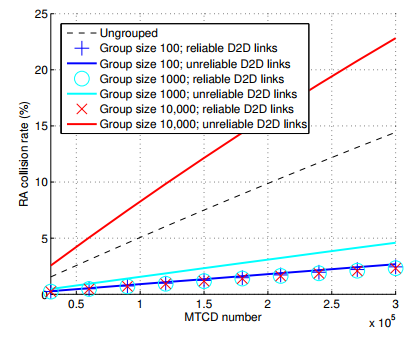
\includegraphics[width=0.8\textwidth]{figures/8.png}
    \setbeamerfont{caption}{size=\tiny}
    \end{figure}
\end{frame}
\section{}
\section{References}
\calcreferencespagetotal % Calc your References Page total number
\begin{frame}[allowframebreaks]{References}
    \fontsize{9pt}{13}\selectfont
    \bibliographystyle{IEEEtran}
    \bibliography{IEEEabrv,Citation}
\end{frame}
\end{document}
